\chapter{Bayesian Logistic Regression Model of 2AFC Discriminability from Experiment 1}
The 2AFC data from Experiment 1 was analyzed with Bayesian Hierarchical Logistic Regression. 

Recall that in this experiment, participants were presented with three stimuli (target, competitor, and decoy rectangles). They were then asked to select the largest rectangle out of a pair of two of these options. There are three trial types: target/competitor (TC), target/decoy (TD), and competitor/decoy (CD). As discussed in the main text, all TC trials and all $TDD = 0\%$ trials were removed from the main analyses.

\section{Model Details} 

The model predicts the probability of discriminating the target/competitor from the decoy option. According to the model, discrimination $D$ for participant $i$ on trial $j$ is:
\begin{align}
    D_{ij} \sim Bernoulli(\theta_{ij})
\end{align}

To compute $\theta_{ij}$, $\eta_{ij}$ is first predicted from a linear combination of the relevant variables.

\begin{align}
\eta_{ij} &= (\beta_{0} + S_{0_{i}}) + (\beta_{\mathrm{or}} + S_{\mathrm{or}_{i}}) \cdot \mathrm{or}_{ij} \\
          &+ (\beta_{\mathrm{horiz}} + S_{\mathrm{horiz}_{i}}) \cdot \mathrm{horiz}_{ij} \\
          &+ (\beta_{\mathrm{TD}} + S_{\mathrm{TD}_{i}}) \cdot \mathrm{TD}_{ij} \\
          &+ (\beta_{\mathrm{TDD5}} + S_{\mathrm{TDD5}_{i}}) \cdot \mathrm{TDD5}_{ij} \\
          &+ (\beta_{\mathrm{TDD9}} + S_{\mathrm{TDD9}_{i}}) \cdot \mathrm{TDD9}_{ij} \\
          &+ (\beta_{\mathrm{TDD14}} + S_{\mathrm{TDD14}_{i}}) \cdot \mathrm{TDD14}_{ij} \\
          &+ (\beta_{\mathrm{TDD5xTD}} + S_{\mathrm{TDD5xTD}_{i}}) \cdot \mathrm{TDD5}_{ij} \cdot \mathrm{TD}_{ij} \\
          &+ (\beta_{\mathrm{TDD9xTD}} + S_{\mathrm{TDD9xTD}_{i}}) \cdot \mathrm{TDD9}_{ij} \cdot \mathrm{TD}_{ij} \\
          &+ (\beta_{\mathrm{TDD14xTD}} + S_{\mathrm{TDD14xTD}_{i}}) \cdot \mathrm{TDD14}_{ij} \cdot \mathrm{TD}_{ij}
\end{align}

All $\beta$ terms are fixed effects, and all $S$ terms are random (participant) effects. $\beta_{or}$ is the fixed effect of orientation, where $\text{or}_{ij}$ is a dummy variable which $=0$ if the target and decoy are taller than wide and $=1$ if the target and decoy are wider than tall. $\beta_{\mathrm{horiz}}$ is the fixed effect of the horizontal display, where $\mathrm{horiz}_{ij}$ is a dummy variable which $=0$ for triangle display trials and $=1$ for horizontal display trials. $\beta_{TD}$ is the fixed effect of comparison, where $TD_{ij}$=0 for CD trials and $TD_{ij}=1$ for TD trials.  The $TDD$ variable has 4 levels ($2\%$, $5\%$, $9\%$, and $14\%$), so there are three dummy variables ($TDD5$, $TDD9$, and $TDD14$) with $2\%$ being the reference level for $TDD$. The interaction captures the additional boost / decrement to $TD$ over $CD$ trials at each level of $TDD$. 

$\eta_{ij}$ is then transformed to the probability scale using the logit function:

\begin{align*}
    \theta_{ij}=\frac{1}{1+e^{-\eta_{ij}}}
\end{align*}

\section{Prior Distributions on Parameters}

\begin{itemize}
    \item $\beta_{0} \sim \mathcal{N}(0,5)$
    \item $\beta_{or} \sim \mathcal{N}(0,5)$
    \item $\beta_{horiz} \sim \mathcal{N}(0,5)$
    \item $\beta_{TD} \sim \mathcal{N}(0,5)$
    \item $\beta_{TDD5} \sim \mathcal{N}(0,5)$
    \item $\beta_{TDD9} \sim \mathcal{N}(0,5)$
    \item $\beta_{TDD14} \sim \mathcal{N}(0,5)$
    \item $\beta_{TDD5xTD} \sim \mathcal{N}(0,2.5)$
    \item $\beta_{TDD9xTD} \sim \mathcal{N}(0,2.5)$
    \item $\beta_{TDD14xTD} \sim \mathcal{N}(0,2.5)$
    \item $S_{0_{i}} \sim \mathcal{N}(0, \sigma_{S_0})$
    \item $S_{or_{i}} \sim \mathcal{N}(0, \sigma_{S})$
    \item $S_{horiz_{i}} \sim \mathcal{N}(0, \sigma_{S})$
    \item $S_{TD_{i}} \sim \mathcal{N}(0, \sigma_{S})$
    \item $S_{TDD5_{i}} \sim \mathcal{N}(0, \sigma_{S})$
    \item $S_{TDD9_{i}} \sim \mathcal{N}(0, \sigma_{S})$
    \item $S_{TDD14_{i}} \sim \mathcal{N}(0, \sigma_{S})$
    \item $S_{TDD5xTD_{i}} \sim \mathcal{N}(0, \sigma_{S})$
    \item $S_{TDD9xTD_{i}} \sim \mathcal{N}(0, \sigma_{S})$
    \item $S_{TDD14xTD_{i}} \sim \mathcal{N}(0, \sigma_{S})$
    \item $\sigma_{S_{0}} \sim \text{LogNormal}(0,2.5)$
    \item $\sigma_{S} \sim \text{LogNormal}(0,2.5)$
\end{itemize}

Note that the model assumes equal variance for all random effect distributions aside from the random intercepts.

\section{Modeling Results}
The model was coded using the Stan programming language \parencite{carpenter2017stan} and implemented with the RStan package \parencite{rstan}. The sampler ran $5$ chains, each for $2500$ iterations. Posterior diagnostics indicated that the sampler converged.

\subsection{Parameter estimates.}

Table~\ref{tab:e1_params} shows parameter estimates, including means and $95\%$ credible intervals. 
\begin{table}[ht]
    \centering
    \begin{tabular}{l r r r r}
        \toprule
        Parameter & M & SD & CI low & CI high \\
        \midrule
        $\beta_{0}$ & 0.44 & 0.06 & 0.32 & 0.57 \\
        $\beta_{or}$ & -0.54 & 0.06 & -0.66 & -0.43\\
        $\beta_{horiz}$ & 0.23 & 0.06 & 0.12 & 0.34\\
        $\beta_{TD}$ & 0.17 & 0.08 & 0.01 & 0.33\\
        $\beta_{TDD5}$ & 0.40 & 0.08 & 0.23 & 0.56\\
        $\beta_{TDD9}$ & 0.81 & 0.09 & 0.64 & 0.98\\
        $\beta_{TDD14}$ & 1.45 & 0.10 & 1.25 & 1.64\\
        $\beta_{TDD5xTD}$ & 0.14 & 0.12 & -0.09 & 0.36\\
        $\beta_{TDD9xTD}$ & 0.61 & 0.13 & 0.36 & 0.85\\
        $\beta_{TDD14xTD}$ & 0.79 & 0.15 & 0.50 & 1.10\\
        $\sigma_{S_0}$ & 0.20 & 0.04 & 0.12 & 0.29 \\
        $\sigma_{S}$ & 0.34 & 0.03 & 0.29 & 0.39 \\
    \bottomrule 
    \end{tabular}
    \caption{Parameter estimates for Bayesian Hierarchical Logistic Regression from Experiment 1 Data, including means, standard deviations, and $95\%$ Credible Intervals.}
    \label{tab:e1_params}
 \end{table}
    
 Inference is made by examining the posterior distributions of the fixed effect parameters (i.e., all $\beta$ values). First, consider the main effects. The intercept $\beta_{0}$ was above $0$, $\textit{M}=0.44, 95\%CI [0.32, 0.57]$, indicating that participants could perform the discrimination task, even at the lowest TDD level. There was also a main effect of orientation, $\textit{M}=-0.54, 95\%CI [-0.66, -0.43]$, indicating that participants performed worse when the target and decoy were oriented wide than when they were oriented tall. The main effect of horizontal, $\textit{M}=0.23, 95\%CI [0.12, 0.34]$, indicates that participants performed better in the horizontal display condition than in the triangle display condition. The main effect of TD comparison was above 0, $\textit{M}=0.17, 95\%CI [0.01, 0.33]$, indicating participants were performed better in target-decoy trials than in competitor decoy trials. 

 Crucially, there was an interaction between comparison (TC vs TD) and TDD. The effect of TD at $TDD=5\%$ was not reliably above 0, $\textit{M}=0.14, 95\%CI [-0.09, 0.36]$. However, the effect of TD at $TDD=9\%$ was above 0, $\textit{M}=0.61, 95\%CI [0.36, 0.85]$, even after accounting for the main effect of TD comparison. The effect of TD at $TDD=14\%$ was also above 0, $\textit{M}=0.79, 95\%CI [0.50, 1.10]$.

\chapter{Bayesian Hierarchical Modeling of Circle Judgment Data from Experiment 2}

The circle judgment data were analyzed with the multivariate Thurstonian perceptual model first presented in Chapter 2. 

\section{Model Details}

The model assumes that, for participant $i$ on trial $j$, the vector of perceived areas $\boldsymbol{X}_{ij}$ is sampled from a multivariate normal distribution with parameters $\boldsymbol{\mu}_{ij}$ and $\boldsymbol{\Sigma}$. That is,
\begin{align}
    \boldsymbol{X}_{ij} \sim \mathcal{N}(\boldsymbol{\mu}_{ij}, \boldsymbol{\Sigma})
\end{align}

Using Bayesian statistical modeling, the parameters $\boldsymbol{\mu}$ and $\boldsymbol{\Sigma}$ were estimated for the model outlined in Chapter 2. Note $\boldsymbol{\mu}$ is allowed to vary systematically over trials and participants, but $\Sigma$ remains constant. $\boldsymbol{\mu}$ is estimated via hierarchical regression while allowing the components of $\boldsymbol{\Sigma}$ (i.e., $\boldsymbol{\sigma_{T}}$, $\boldsymbol{\sigma_{C}}$, $\boldsymbol{\sigma_{D}}$, $\rho_{TD}$, $\rho_{TC}$, $\rho_{CD}$) to vary freely. 

The model was fit separately for the triangle and horizontal condition. First, the computation of $\boldsymbol{\mu}$ is described, followed by the computation $\boldsymbol{\Sigma}$. Tthe prior distributions on each parameter separately for each of these components are shown, followed by an explanation of the modeling procedure and results. Note that the model predicts mean-centered log-transformed estimated area.

\subsection{\texorpdfstring{$\boldsymbol{\mu}$}{mu} Parameterization}

The model predicts the mean area $\mu_{ijk}$ for the $i$th participant on the $j$th trial for the $k$th stimulus. There were $k=3$ stimuli on each trial. If $k=1$, the stimulus is the target; If $k=2$, the stimulus is the competitor; If $k=3$, the stimulus is the decoy. Thus, $\boldsymbol{\mu}$ can be broken down into $\mu_{ij1}$ (target), $\mu_{ij2}$ (competitor), and $\mu_{ij3}$ (decoy). Note that some parameters are common to all stimuli (e.g., the effects of diagonal or orientation), while others are common only to a particular option (e.g., the effect of competitor vs. decoy vs. target). 

$\mu_{ij1}$ is computed as:

\begin{equation}
    \begin{aligned}
        \mu_{ij1}=(S_{0_i} + \beta_{0}) + \beta_{or} \cdot \mathrm{or}_{ij1} + \beta_{\mathrm{diag}2} \cdot \mathrm{diag}2_{ij}+ \\
        \beta_{\mathrm{diag}3} \cdot \mathrm{diag}3_{ij} + \beta_{\mathrm{TDD}5} \cdot \mathrm{TDD}5_{ij} +\\ \beta_{\mathrm{TDD}9} \cdot \mathrm{TDD}9_{ij} + \beta_{\mathrm{TDD}14} \cdot \mathrm{TDD}14_{ij}
        \label{circle_mu_eqn1}
    \end{aligned}
\end{equation}

$S_{0_i}$ is a random intercept for participant $i$. $\beta_{0}$ is the fixed intercept. $\beta_{or}$ is the fixed effect of orientation, where $or_{ij1}$ is a dummy variable which $=0$ if the target is taller than wide and $=1$ if the target is wider than tall. $\beta_{diag2}$ is the fixed effect of the middle diagonal, which $=1$ if the all stimuli on the trial fall on the middle diagonal and $=0$ otherwise. $\beta_{diag3}$ is the fixed effect of the upper diagonal, which $=1$ if all stimuli on the trial fall on the upper diagonal and $=0$ otherwise. $\beta_{TDD5}$ is the fixed effect of TDD 5, and $TDD5_{ij}$ is a dummy variable which $=1$ if $TDD=5\%$ and $=0$ otherwise. $\beta_{TDD9}$ is the fixed effect of TDD 9, and $TDD9_{ij}$ is a dummy variable which $=1$ if $TDD=9\%$ and $=0$ otherwise. $\beta_{TDD14}$ is the fixed effect of TDD 14, and $TDD14_{ij}$ is a dummy variable which $=1$ if $TDD=14\%$ and $=0$ otherwise. 

$\mu_{ij2}$ is computed as:

\begin{equation}
    \begin{aligned}
        \mu_{ij2}=(S_{0_i} + \beta_{0}) + \beta_{\mathrm{or}} \cdot \mathrm{or}_{ij2} + \beta_{\mathrm{diag}2} \cdot \mathrm{diag}2_{ij}+ \\\beta_{\mathrm{diag}3} \cdot \mathrm{diag}3_{ij} + \beta_{\mathrm{TDD}5} \cdot \mathrm{TDD}5_{ij} + \\\beta_{\mathrm{TDD}9} \cdot \mathrm{TDD}9_{ij} + \beta_{\mathrm{TDD}14} \cdot \mathrm{TDD}14_{ij} + \beta_{\mathrm{comp}}
        \label{circle_mu_eqn2}
    \end{aligned}
\end{equation}

$S_{0_i}$ is a random intercept for participant $i$. $\beta_{0}$ is the fixed intercept. $\beta_{or}$ is the fixed effect of orientation, where $or_{ij2}$ is a dummy variable which $=0$ if the competitor is taller than wide and $=1$ if the competitor is wider than tall. $\beta_{diag2}$ is the fixed effect of the middle diagonal, which $=1$ if the all stimuli on the trial fall on the middle diagonal and $=0$ otherwise. $\beta_{diag3}$ is the fixed effect of the upper diagonal, which $=1$ if all stimuli on the trial fall on the upper diagonal and $=0$ otherwise. $\beta_{TDD5}$ is the fixed effect of TDD 5, and $TDD5_{ij}$ is a dummy variable which $=1$ if $TDD=5\%$ and $=0$ otherwise. $\beta_{TDD9}$ is the fixed effect of TDD 9, and $TDD9_{ij}$ is a dummy variable which $=1$ if $TDD=9\%$ and $=0$ otherwise. $\beta_{TDD14}$ is the fixed effect of TDD 14, and $TDD14_{ij}$ is a dummy variable which $=1$ if $TDD=14\%$ and $=0$ otherwise. $\beta_{comp}$ is a parameter that reflects the possibility of estimation bias for the competitor.

$\mu_{ij3}$ is computed as:

\begin{equation}
    \begin{aligned}
        \mu_{ij3}=(S_{0_i} + \beta_{0}) + \beta_{\mathrm{or}} \cdot \mathrm{or}_{ij3} + \beta_{\mathrm{diag}2} \cdot \mathrm{diag}2_{ij}+ \\\beta_{\mathrm{diag}3} \cdot \mathrm{diag}3_{ij} + (\beta_{\mathrm{TDD}5} + \beta_{\mathrm{TDD}5D}) \cdot \mathrm{TDD}5D_{ij} + (\beta_{\mathrm{TDD}9} + \beta_{\mathrm{TDD}9D}) \cdot \mathrm{TDD}9D_{ij} +\\ (\beta_{\mathrm{TDD}14} +\\ \beta_{\mathrm{TDD}14D}) \cdot \mathrm{TDD}14D_{ij}
        \label{circle_mu_eqn3}
    \end{aligned}
\end{equation}

$S_{0_i}$ is a random intercept for participant $i$. $\beta_{0}$ is the fixed intercept. $\beta_{or}$ is the fixed effect of orientation, where $or_{ij3}$ is a dummy variable which $=0$ if the decoy is taller than wide and $=1$ if the decoy is wider than tall. $\beta_{diag2}$ is the fixed effect of the middle diagonal, which $=1$ if the all stimuli on the trial fall on the middle diagonal and $=0$ otherwise. $\beta_{diag3}$ is the fixed effect of the upper diagonal, which $=1$ if all stimuli on the trial fall on the upper diagonal and $=0$ otherwise. $\beta_{TDD2D}$ is the fixed effect of TDD=2, and $TD25D_{ij}$ is a dummy variable which $=1$ if $TDD=2\%$ for the decoy and $=0$ otherwise.  $\beta_{TDD5D}$ is the fixed effect of TDD=5, and $TDD5D_{ij}$ is a dummy variable which $=1$ if $TDD=5\%$ for the decoy and $=0$ otherwise. $\beta_{TDD9D}$ is the fixed effect of TDD 9 for the decoy, and $TDD9D_{ij}$ is a dummy variable which $=1$ if $TDD=9\%$ and $=0$ otherwise. $\beta_{TDD14D}$ is the fixed effect of TDD 14 for the decoy, and $TDD14D_{ij}$ is a dummy variable which $=1$ if $TDD=14\%$ and $=0$ otherwise. 

Note that there is a common set of parameters for each level of TDD and additional set of parameters for each level of TDD that only apply to the decoy. In the data, it was clear that participants often adjusted the target and competitor relative to the decoy. In other words, even though the physical size of both target and competitor remains constant across TDD, participants' \textit{estimation} of their size varied with TDD. The inclusion of a separate set of parameters for TDD that only apply to the decoy allows for a "deflection" of the decoy size, relative to target and competitor size. 

Note the following reference points for the variables:
\begin{itemize}
    \item TDD: $2\%$
    \item Orientation: taller than wide
    \item Diagonal: lower
    \item Stimulus: target
\end{itemize}

The $\beta_{0}$ parameter captures the fixed of a tall target on the lower diagonal at $2\%$ TDD, and all other parameters reflect deflections from this.

\subsubsection{Prior Distributions on Parameters}
Below are shown the following prior distributions on each parameter relevant to $\boldsymbol{\mu}$:
\begin{itemize}
    \item $\beta_{0} \sim \mathcal{N}(0,5)$
    \item $\beta_{or} \sim \mathcal{N}(0,5)$
    \item $\beta_{diag2} \sim \mathcal{N}(0,5)$
    \item $\beta_{diag3} \sim \mathcal{N}(0,5)$
    \item $\beta_{TDD5} \sim \mathcal{N}(0,5)$
    \item $\beta_{TDD9} \sim \mathcal{N}(0,5)$
    \item $\beta_{TDD14} \sim \mathcal{N}(0,5)$
    \item $\beta_{TDD2D} \sim \mathcal{N}(0,5)$
    \item $\beta_{TDD5D} \sim \mathcal{N}(0,5)$
    \item $\beta_{TDD9D} \sim \mathcal{N}(0,5)$
    \item $\beta_{TDD14D} \sim \mathcal{N}(0,5)$
    \item $\beta_{comp} \sim \mathcal{N}(0,5)$
    \item $S_{0_i} \sim \mathcal{N}(0,\sigma_{S_0})$
    \item $\sigma_{S_0} \sim \text{Half-Cauchy}(0, 2.5)$
\end{itemize}

\section{$\boldsymbol{\Sigma}$ Parameterization}
$\Sigma$ is a positive semi-definite $3\text{x}3$ covariance matrix computed as:

\begin{align}
   \boldsymbol{\Sigma}=S\boldsymbol{\Omega}S
   \label{eqn:Sigma}
\end{align}

where $S$ is a diagonal matrix consisting of: 

\begin{align}
   \begin{pmatrix}
      \sigma_{T} & 0 & 0 \\
      0 & \sigma_{C} & 0 \\
      0 & 0 & \sigma_{D} \\
   \end{pmatrix}
   \label{eqn:S_1}
\end{align}

and $\boldsymbol{\Omega}$ is a correlation matrix:

\begin{align}
   \begin{pmatrix}
      1 & \rho_{TC} & \rho_{TD} \\
      \rho_{TC} & 1 & \rho_{CD} \\
      \rho_{TD} & \rho_{CD} & 1 \\
   \end{pmatrix}
   \label{eqn:O_1}
\end{align}

Estimation of $S$ was straightforward. The three standard deviation parameters $\sigma_{T}$, $\sigma_{C}$, and $\sigma_{D}$ were freely estimated.

When estimating $\boldsymbol{\Omega}$, the LKJ distribution \parencite{lewandowski2009generating} was used to set priors on the Cholesky factorization of the correlation matrix $\Omega$. This was done to ensure that the resulting variance-covariance matrix $\boldsymbol{\Sigma}$ is positive semi-definite, a requirement of the multivariate Gaussian distribution. The critical inferences, however, are performed on the off-diagonal elements $\rho_{TC}$, $\rho_{TD}$, $\rho_{CD}$ in each display condition. Priors were set on the $\sigma$ parameters using the Half-Cauchy distribution \parencite{gelman2006prior}. 

\subsection{Prior Distributions on Parameters}
Below are shown the following prior distributions on each parameter relevant to $\boldsymbol{\Sigma}$.
\begin{itemize}
    \item $\sigma_{T} \sim\text{Half-Cauchy}(0,2.5)$
    \item $\sigma_{C} \sim\text{Half-Cauchy}(0,2.5)$
    \item $\sigma_{D} \sim\text{Half-Cauchy}(0,2.5)$
    \item $\boldsymbol{\Omega} \sim \text{LKJCorr}(\eta=1)$
\end{itemize}

\section{Modeling Results}
The model was implemented using the Stan programming language \parencite{carpenter2017stan} using the cmdstanr interface \parencite{cmdstanr} in R . 

The model ran for 2500 iterations (not including warm-up) with 4 chains for each display condition. Posterior diagnostics indicated that the sampler converged in each condition.

Below are parameter estimates for each display condition and relevant parameter. The estimates of the participant effects $S_{0_i}$ are excluded for brevity. Estimates are rounded to two or three decimal places, depending on the size of the parameter.
    
\begin{table}[ht]
    \centering
    \begin{tabular}{llrrrr}
        \toprule
        Display Condition & Parameter & \textit{M} & \textit{SD} & HDI lower & HDI upper \\
        \midrule
        \textbf{Horizontal}  &  $\beta_{0}$     &    $-0.41$   &   $0.02$    &  $-0.44$     & $-0.38$     \\
                    &  $\beta_{or}$    &    $0.003$   &   $0.002$   &  $-0.001$    & $0.007$     \\
                    &  $\beta_{diag2}$ &    $0.47$    &   $0.01$    &  $0.46$      & $0.48$      \\
                    &  $\beta_{diag3}$ &    $0.80$    &   $0.01$    &  $0.79$      & $0.81$      \\
                    &  $\beta_{TDD5}$  &    $-0.005$  &   $0.01$    &  $-0.017$    & $0.007$     \\
                    &  $\beta_{TDD9}$  &    $-0.007$  &   $0.01$    &  $-0.019$    & $0.005$     \\
                    &  $\beta_{TDD14}$ &    $-0.01$   &   $0.01$    &  $-0.02$     & $-0.0005$   \\
                    &  $\beta_{TDD2D}$ &    $-0.006$  &   $0.004$   &  $-0.013$    & $0.001$     \\
                    &  $\beta_{TDD5D}$ &    $-0.01$   &   $0.004$   &  $-0.016$    & $-0.003$    \\
                    &  $\beta_{TDD9D}$ &    $-0.04$   &   $0.004$   &  $-0.05$     & $-0.04$     \\
                    &  $\beta_{TDD14D}$&    $-0.08$   &   $0.004$   &  $-0.09$     & $-0.07$     \\
                    &  $\beta_{comp}$  &    $0.003$   &   $0.002$   &  $-0.002$    & $0.007$     \\
                    &  $\sigma_{S_0}$  &    $0.19$    &   $0.01$    &  $0.17$      & $0.21$      \\
                    &  $\sigma_{T}$    &    $0.337$   &   $0.002$   &  $0.334$     & $0.340$     \\
                    &  $\sigma_{C}$    &    $0.341$   &   $0.002$   &  $0.338$     & $0.345$     \\
                    &  $\sigma_{D}$    &    $0.337$   &   $0.002$   &  $0.333$     & $0.340$     \\
                    &  $\rho_{TC}$     &    $0.575$   &   $0.005$   &  $0.565$     & $0.584$     \\
                    &  $\rho_{TD}$     &    $0.710$   &   $0.004$   &  $0.703$     & $0.716$     \\
                    &  $\rho_{CD}$     &    $0.575$   &   $0.005$   &  $0.565$     & $0.584$     \\
        \textbf{Triangle}    &  $\beta_{0}$     &    $-0.40$   &   $0.01$    &  $-0.42$     & $-0.38$     \\
                    &  $\beta_{or}$    &    $-0.006$  &   $0.002$   &  $-0.01$     & $-0.002$    \\
                    &  $\beta_{diag2}$ &    $0.47$    &   $0.005$   &  $0.455$     & $0.474$     \\
                    &  $\beta_{diag3}$ &    $0.81$    &   $0.005$   &  $0.80$      & $0.82$      \\
                    &  $\beta_{TDD5}$  &    $-0.01$   &   $0.006$   &  $-0.03$     & $0.0003$    \\
                    &  $\beta_{TDD9}$  &    $-0.02$   &   $0.006$   &  $-0.03$     & $-0.008$    \\
                    &  $\beta_{TDD14}$ &    $-0.03$   &   $0.006$   &  $-0.04$     & $-0.01$     \\
                    &  $\beta_{TDD2D}$ &    $-0.0172$ &   $0.004$   &  $-0.024$    & $-0.01$     \\
                    &  $\beta_{TDD5D}$ &    $-0.0167$ &   $0.004$   &  $-0.0237$   & $-0.01$     \\
                    &  $\beta_{TDD9D}$ &    $-0.03$   &   $0.004$   &  $-0.037$    & $-0.02$     \\
                    &  $\beta_{TDD14D}$&    $-0.05$   &   $0.004$   &  $-0.06$     & $-0.05$     \\
                    &  $\beta_{comp}$  &    $0.005$   &   $0.002$   &  $0.0001$    & $0.009$     \\
                    &  $\sigma_{S_0}$  &    $0.15$    &   $0.01$    &  $0.14$      & $0.17$      \\
                    &  $\sigma_{T}$    &    $0.335$   &   $0.002$   &  $0.332$     & $0.338$     \\
                    &  $\sigma_{C}$    &    $0.338$   &   $0.002$   &  $0.335$     & $0.341$     \\
                    &  $\sigma_{D}$    &    $0.335$   &   $0.002$   &  $0.331$     & $0.338$     \\
                    &  $\rho_{TC}$     &    $0.541$   &   $0.005$   &  $0.531$     & $0.551$     \\
                    &  $\rho_{TD}$     &    $0.675$   &   $0.004$   &  $0.667$     & $0.682$     \\
                    &  $\rho_{CD}$     &    $0.533$   &   $0.005$   &  $0.523$     & $0.543$     \\
        \bottomrule
    \end{tabular}
    \caption{Parameter estimates for Bayesian Hierarchical Thurstonian Model from Experiment 2 Circle Phase Data, including means, standard deviations, and $95\%$ Credible Intervals.}
    \label{tab:e2_params}
\end{table}

The posterior estimates indicate that $\rho_{TD}>\rho_{TC}\approx\rho_{CD}$ in each display condition, in accordance with the predictions. Furthermore, the absolute values of all $\rho$ values are greater in the horizontal condition than in the triangle condition, suggesting that the horizontal condition better facilitates comparisons. 

The $\beta$ estimates are generally as expected. The $\beta_{diag}$ estimates show that participants increased their area estimations with the absolute size of the stimuli. Participants also decreased the size of decoy estimations as TDD increased. They also, to some extent, decreased the size of target and competitor estimations as TDD increased (captured by the $\beta_{TDD5}$, $\beta_{TDD9}$, and $\beta_{TDD14}$) parameters, indicating that participants adjusted the target and competitor relative to the decoy.

Interestingly, the $\beta_{or}$ estimates indicated that participants rated wider stimuli larger than tall stimuli in the horizontal condition, but they rated taller stimuli larger than wide stimuli in the horizontal condition. This effect is quite small, but is nonetheless present in the parameter estimates.

Participants also rated the competitor slightly larger than the target, particularly in the triangle condition, although this effect is quite small. This effect was indeed to small to show differences in any single TDD level (see Figure~\ref{fig:e2mu}). 

\chapter{Inferential Statistics for Experiment 2 Choice Data}

Following \textcite{katsimpokisRobustBayesianTest2022}, I performed inference on \textit{Absolute Share of the Target}, a variant of RST that corrects for a bias in RST. AST is an unweighted average of the target choice proportion from each choice set. Here, AST is computed as:

\begin{equation}
    \begin{aligned}
        AST=0.5 \cdot (\frac{P(H|{H,W,D_{H}})}{P(H|{H,W,D_{H}})+P(W|{H,W,D_{H}})}+ \\
        \frac{P(W|{H,W,D_{W}})}{P(W|{H,W,D_{W}})+P(H|{H,W,D_{W}})})
    \end{aligned}
\end{equation}

AST was computed for each participant in each display condition at each level of TDD. First are the analyses from the triangle condition followed by those from the horizontal condition. 

\section{Triangle Condition Analysis}
A one-way within-groups ANOVA testing the effect of TDD on AST in the triangle condition was significant, $\textit{F}(3,636)=79.97$,$\textit{p}<.001$. 

I then performed a follow-up one-sample t-test on AST at each level of TDD, using the within-participants error correction from \textcite{cousineau2014error} and comparing the mean AST value to the null value $.5$. I compared each p-value to a Bonferroni-corrected $\alpha$ level of $\alpha=\frac{.05}{4}=.0125$. 

The AST value was significantly different from $.5$ at TDD=$2\%$, $\textit{t}(212)=-18.4,\textit{p}<.001$, $\textit{M}=.34$, $95\%\text{CI}[.33,.36]$, indicating a repulsion effect. 

The AST value was significantly different from $.5$ at TDD=$5\%$, $\textit{t}(212)=-13.2,\textit{p}<.001$, $\textit{M}=.39$, $95\%\text{CI}[.38,.41]$, indicating a repulsion effect. 

The AST value was significantly different from $.5$ at TDD=$9\%$, $\textit{t}(212)=-7.45,\textit{p}<.001$, $\textit{M}=.43$, $95\%\text{CI}[.42,.45]$, indicating a repulsion effect. 

The AST value was significantly different from $.5$ at TDD=$14\%$, $\textit{t}(212)=-2.34,\textit{p}=.002$, $\textit{M}=.48$, $95\%\text{CI}[.46,.49]$, indicating a slight repulsion effect. Note that the mean $P(T)>P(C)$ in Figure~\ref{fig:e2_choiceprops}; however, those values are not equally weighted.

\section{Horizontal Condition Analysis}
IA one-way within-groups ANOVA testing the effect of TDD on AST in the horizontal condition was significant, $\textit{F}(3,618)=176.10$,$\textit{p}<.001$. 

I then performed a follow-up one-sample t-test on AST at each level of TDD, using the within-participants error correction from \textcite{cousineau2014error} and comparing the mean AST value to the null value $.5$. Each p-value was compared to a Bonferroni-corrected $\alpha$ level of $\alpha=\frac{.05}{4}=.0125$. 

The AST value was significantly different from $.5$ at TDD=$2\%$, $\textit{t}(206)=-15.6,\textit{p}<.001$, $\textit{M}=.34$, $95\%\text{CI}[.33,.36]$, indicating a repulsion effect. 

The AST value was significantly different from $.5$ at TDD=$5\%$, $\textit{t}(206)=-8.12,\textit{p}<.001$, $\textit{M}=.41$, $95\%\text{CI}[.39,.43]$, indicating a repulsion effect. 

The AST value was not significantly different from $.5$ at TDD=$9\%$, $\textit{t}(206)=-0.04,\textit{p}=.10$, $\textit{M}=.50$, $95\%\text{CI}[.48,.52]$, indicating a null effect. 

The AST value was significantly different from $.5$ at TDD=$14\%$, $\textit{t}(206)=5.00,\textit{p}<.001$, $\textit{M}=.56$, $95\%\text{CI}[.54,58]$, indicating an attraction effect. 

Mean AST values for each TDD level in each display condition are plotted in Figure~\ref{fig:e2_ast}.

\begin{figure}
   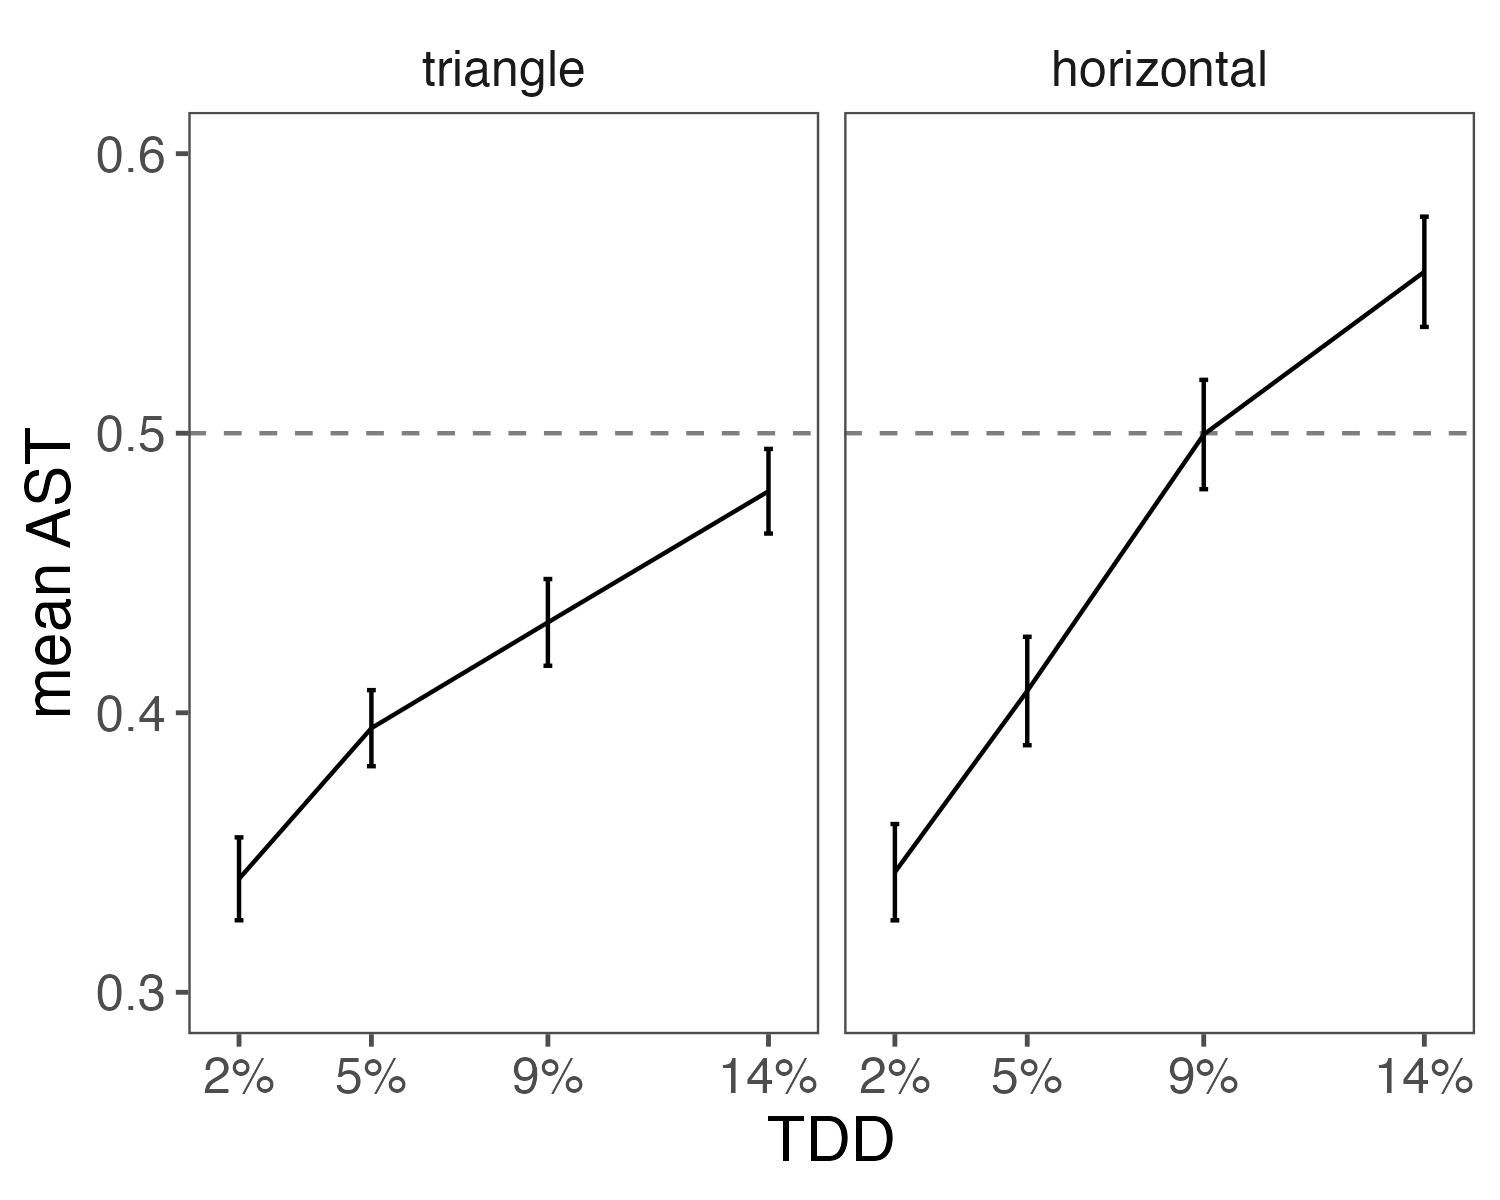
\includegraphics[width=100mm]{figures/choicePhase_mean_ast.jpeg}
   \caption{Mean AST values for each display condition and TDD level from Experiment 2. Error bars are $95\%$ CIs with the within-participants error correction from \textcite{cousineau2014error}.}
   \label{fig:e2_ast}
\end{figure}

\chapter{Maxdiff Modeling from Experiment 3}
According to the maxdiff model of best-worst choice \parencite{marleyProbabilisticModelsBest2005}, the probability $BW_{K}(x,y)$ of selecting option $x$ as best and $y$ as worst from choice set $K$ is computed as:

\begin{equation}
   BW_{K}(x,y)=\frac{e^{u_{x}-u_{y}}}{\sum_{\substack{{p,q}\in K\\p \neq q}} e^{u_{p}-u_{q}}}   
   \label{eqn:maxdiff_equation1}
\end{equation}

where $u_{i}$ is the utility of option $i$. 

Below are the details of the maxdiff modeling, as applied to the data from Experiment 3.

\section{Model Details}
Following typical approaches in the choice modeling literature, the utility of each option in a choice set was estimated using linear regression. There was no intercept.

According the model, the utility $U_{ijk}$ for participant $i$ on trial $j$ and option $k$ is computed as:

\begin{equation}
    \begin{aligned}
        U_{ijk}=\beta_{or} \cdot \mathrm{or}_{ijk} + \beta_{\mathrm{TDD}5} \cdot \mathrm{TDD}5_{ij} +\beta_{\mathrm{TDD}9} \cdot \mathrm{TDD}9_{ij} + \beta_{\mathrm{TDD}14} \cdot \mathrm{TDD}14_{ij}+\\
        (\beta_{comp}+S_{comp_i}) \cdot comp_{ijk}+(\beta_{decoy}+S_{decoy_i}) \cdot decoy_{ijk}+
        \label{maxdiff_U}
    \end{aligned}
\end{equation}

As in the modeling of Experiment 2, there was an effect of option (i.e., target, competitor, decoy) where $\beta_{comp}$ and $S_{comp_i}$ are the fixed and random effects for the competitor stimulus, respectively, and $comp_{ijk}$ is a dummy variable which equals 1 if the stimulus is a competitor and 0 otherwise. Similarly, $\beta_{decoy}$ and $S_{decoy_i}$ are the fixed and random effects for the decoy stimulus, respectively, and $comp_{ijk}$ is a dummy variable which equals 1 if the stimulus is a decoy and 0 otherwise. Note that the reference level is the target here. These analyses collapse over diagonal.

According to the model, the probability a participant $i$ on trial $j$, given set $K$, selects option $k$ as best and $l$ as worst, $k \neq l$, is computed as:

\begin{align}
    BW_{ij_{K}}(k,l)=\frac{e^{U_{ijk}-U_{ijl}}}{\sum_{\substack{{p,q}\in K\\p \neq q}} e^{u_{p}-u_{q}}}
\end{align}

The vector $\boldsymbol{\theta_{ij}}$ is a vector of all possible best-worst choices for participant $i$ and trial $j$, where $\sum \boldsymbol{\theta_{ij}} = 1$.

The count vector of all possible BW choices $\boldsymbol{C_{ij}}$ is distributed:

\begin{align}
    \boldsymbol{C}_{ij} \sim \text{Multinomial}(\boldsymbol{\theta}_{ij})
\end{align}


Below are the prior distributions on all parameters.

\section{Prior Distributions on Parameters}
\begin{itemize}
    \item $\beta_{or} \sim \mathcal{N}(0, 5)$
    \item $\beta_{TDD5} \sim \mathcal{N}(0, 5)$
    \item $\beta_{TDD9} \sim \mathcal{N}(0, 5)$
    \item $\beta_{TDD14} \sim \mathcal{N}(0, 5)$
    \item $\beta_{comp} \sim \mathcal{N}(0, 5)$
    \item $\beta_{decoy} \sim \mathcal{N}(0, 5)$
    \item $\beta_{S_comp_i} \sim \mathcal{N}(0, \sigma_{S_comp})$
    \item $\beta_{S_decoy_i} \sim \mathcal{N}(0, \sigma_{S_decoy})$
    \item $\sigma_{S_comp} \sim \text{Half-Cauchy}(0, 2.5)$
    \item $\sigma_{S_comp} \sim \text{Half-Cauchy}(0, 2.5)$
\end{itemize}

\section{Parameter Estimates}
Table~\ref{tab:maxdiff_params} shows parameter estimates, including means and $95\%$ credible intervals. 
\begin{table}[ht]
    \centering
    \begin{tabular}{lrrrr}
        \toprule
        Parameter & M & SD & CI low & CI high \\
        \midrule
        $\beta_{or}$ & 0.27 & 0.01 & 0.26 & 0.28\\
        $\beta_{TDD5}$ & 0.27 & 0.01 & 0.24 & 0.29\\
        $\beta_{TDD9}$ & 0.64 & 0.01 & 0.61 & 0.67\\
        $\beta_{TDD14}$ & 1.05 & 0.02 & 1.02 & 1.08\\
        $\beta_{comp}$ & -0.03 & 0.01 & -0.05 & -0.01\\
        $\beta_{decoy}$ & -0.25 & 0.02 & -0.28 & -0.21\\
        $\sigma_{comp}$ & 0.14 & 0.01 & 0.12 & 0.16 \\
        $\sigma_{decoy}$ & 0.29 & 0.01 & 0.27 & 0.32 \\
        \bottomrule 
    \end{tabular}
    \caption{Parameter estimates for maxdiff modeling from Experiment 3, including means, SDs, and $95\%$ Credible Intervals.}
    \label{tab:maxdiff_params}
 \end{table}

\chapter{Bayesian Modeling of Price Data from Experiment 4}

The pricing data from Experiment 4 were modeled using the Thurstonian model from of Experiment 2.

\section{Thurstonian Price Model}

The model assumed that on each trial $i$, a vector of prices $\textbf{X}_{i}$ is drawn of a multivariate normal distribution:

\begin{align}
    \textbf{X}_{i}\sim \mathcal{\textbf{N}}(\boldsymbol{\mu}_{jk},\boldsymbol{\Sigma}_{k})
\end{align}

where $j$ is the product category (washing machines, laptops, televisions, microwave ovens) and $k$ is the trial type (attraction, repulsion). 

$\boldsymbol{\mu}_{jk}$ is the column vector:

\begin{align}
   \begin{pmatrix}
      \mu_{T_jk} \\
      \mu_{C_jk} \\
      \mu_{D_jk}
\end{pmatrix}
   \label{eqn:mu_price}
\end{align}

and $\boldsymbol{\Sigma}_{k}$ is a $3\text{x}3$ positive semi-definite variance-covariance matrix:

\begin{align}
   \boldsymbol{\Sigma}_{k}=S\boldsymbol{\Omega}_{k}S
\end{align}

where $S$ is a diagonal matrix consisting of: 

\begin{align}
   \begin{pmatrix}
      \sigma_{T} & 0 & 0 \\
      0 & \sigma_{C} & 0 \\
      0 & 0 & \sigma_{D} 
   \end{pmatrix}
\end{align}

with $\sigma_{T}$, $\sigma_{C}$, $\sigma_{D}$ being the standard deviations for target, competitor, and decoy, respectively. $\boldsymbol{\Omega}_{k}$ is a correlation matrix:

\begin{align}
   \begin{pmatrix}
      1 & \rho_{TC_k} & \rho_{TD_k} \\
      \rho_{TC_k} & 1 & \rho_{CD_k} \\
      \rho_{TD_k} & \rho_{CD_k} & 1 
   \end{pmatrix}
\end{align}

with $\rho_{TD_1}$, for example, indicating the population-level correlation between target and decoy valuations in the attraction condition.

This model has relatively $24$ free parameters,relatively few compared to the several hundred from Experiment 2.

There were no a priori predictions about the size or even direction of the price differences here. All $\boldsymbol{\mu}$ parameters were freely estimated rather than estimated through linear regression as in Experiment 2.

Prior to model estimation, all prices were normalized within participants. 

\section{Prior Distributions on all Parameters}

\begin{itemize}
    \item $\boldsymbol{\mu}_{jk} \sim \mathcal{\textbf{N}}(0,1)$
    \item $\sigma_{T} \sim \text{Half-Cauchy}(0,2.5)$
    \item $\sigma_{C} \sim \text{Half-Cauchy}(0,2.5)$
    \item $\sigma_{D} \sim \text{Half-Cauchy}(0,2.5)$
    \item $\boldsymbol{\Omega_{k}} \sim \text{LKJCorr}(\eta=0.5)$
\end{itemize}

\section{Parameter Estimates}

For brevity, the $\boldsymbol{\mu}$ and $\sigma$ estimates are omitted. $\rho$ estimates are shown below.
\begin{table}[ht]
    \centering
    \begin{tabular}{llrrrr}
        \toprule
        Trial Type & Parameter & \textit{M} & \textit{SD} & HDI lower & HDI upper \\
        \midrule
        \textbf{Attraction}  &  $\rho_{TC}$     &    $.87$   &   $0.005$    &  $.86$     & $.88$     \\
                             &  $\rho_{TD}$    &     $.87$   &   $0.005$    &  $.86$     & $.88$     \\
                             &  $\rho_{CD}$    &     $.83$   &   $0.007$    &  $.81$     & $.84$     \\
        \textbf{Repulsion}   &  $\rho_{TC}$     &    $.77$   &   $0.008$    &  $.75$     & $.79$     \\
                             &  $\rho_{TD}$    &     $.87$   &   $0.005$    &  $.86$     & $.88$     \\
                             &  $\rho_{CD}$    &     $.69$   &   $0.011$     &  $.67$     & $.72$     \\
        \bottomrule
    \end{tabular}
    \caption{$\rho$ Parameter estimates for $\rho$ parameters from the Bayesian Hierarchical Thurstonian Model from Experiment 4 Pricing Data, including means, standard deviations, and $95\%$ Credible Intervals.}
    \label{tab:e4_rho_params}
\end{table}

\chapter{Bayesian Modeling of Choice Data from Experiment 4}

The choice data of Experiment 4 were analyzed with a Dirichlet-Multinomial model. The Dirichlet distribution is a generalization of the Beta distribution to $>2$ dimensions. Here the Dirichlet distribution is used to model the variability in ternary choice proportions for the attraction and repulsion trials from Experiment 4.

In this analysis collapsed over participants. This is a limitation, particularly given recent concerns about participant-level variability in context effects \parencite{liewAppropriacyAveragingStudy2016b,trueblood2015fragile}. However, given that the main goal of Experiment 4 was to measure correlations in pricing, and that participants made relatively few choices, this analysis was performed on aggregate choice data.

\section{Dirichlet-Multinomial Choice Model}

According to the model, the vector $\boldsymbol{C_{ijkl}}$ of target, competitor, and decoy counts for trial type (attraction, repulsion) $i$, TDD (near, far) $j$, product category (laptops, microwave ovens, televisions, wachine machines)  $k$, target high dimension (1,2) $l$ is distributed:

\begin{align}
    C_{ijkl} \sim \text{Multinomial}(\boldsymbol{\theta_{ijkl}})
\end{align}

$\boldsymbol{\theta_{ijkl}}$ is a vector of choice probabilities which is turn distributed:

\begin{align}
    \boldsymbol{\theta_{ijkl}} \sim \text{Dirichlet}(\boldsymbol{\alpha_{ijkl}})
\end{align}

where all $\boldsymbol{\alpha}_{ijkl}>0$. 

For a prior distribution on $\boldsymbol{\alpha}$, it was assumed that:

\begin{align}
    \boldsymbol{\alpha_{ijkl}} \sim \text{LogNormal}(1,1)
\end{align}

Inference was performed using the mean target, competitor, and decoy choice probabilities, collapsed across product category and the target's high dimension. See Table~\ref{tab:e4_choice_params}.

\begin{table}[ht]
    \centering
    \begin{tabular}{lllrrr}
        \toprule
        \textbf{Trial Type} & \textbf{TDD} & \textbf{Option} & \textit{M} & HDI lower & HDI upper \\
        Attraction          & Near         & Target          &  $.48$     & $.45$     & $.51$     \\
                            &              & Competitor      &  $.47$     & $.44$     & $.50$     \\
                            &              & Decoy           &  $.05$     & $.03$     & $.06$     \\
                            & Far          & Target          &  $.46$     & $.43$     & $.49$     \\
                            &              & Competitor      &  $.48$     & $.45$     & $.51$     \\
                            &              & Decoy           &  $.07$     & $.05$     & $.08$     \\
        Repulsion           & Near         & Target          &  $.31$     & $.28$     & $.34$     \\
                            &              & Competitor      &  $.66$     & $.63$     & $.69$     \\
                            &              & Decoy           &  $.04$     & $.03$     & $.05$     \\
                            & Far          & Target          &  $.33$     & $.30$     & $.36$     \\
                            &              & Competitor      &  $.65$     & $.62$     & $.68$     \\
                            &              & Decoy           &  $.03$     & $.02$     & $.04$     \\
        \bottomrule
    \end{tabular}
    \caption{Experiment 4 Mean Posterior Choice Proportions from the Bayesian Dirichlet-Multinomial Model.}
    \label{tab:e4_choice_params}
\end{table}

On average, participants chose the competitor more than the target in both TDD levels, in the repulsion effect trials. In the attraction effect trials, participants chose the target and competitor at equal rates. 

\chapter{Bayesian Hierarchical Logistic Regression for Experiment 5 Data}

The comparability data from Experiment 5 were analyzed with a Bayesian hierarchical logistic regression model.

All trials where participants chose the decoy option were removed. Trials where the W and H rectangles were in the first two positions were also removed. 

The target was classified as the option aligned with the decoy in the two-aligned option. The model predicted choice via a linear combination of an intercept, the configuration (none-aligned, two-aligned, all-aligned) and whether the target was in the middle position (1, 0). The reference level for configuration was none-aligned. There were no interactions included in the model. There was also a random effect of participant included in the model. 

The model was fit as a Bayesian hierarchical logistic regression model using the rstanarm package \parencite{rstanarm}, using default priors for all parameters. Posterior estimates for all fixed effects are shown in Table~\ref{tab:e5_logit_params}.

\begin{table}[ht]
    \centering
    \begin{tabular}{lrrrr}
        \toprule
        \textbf{Parameter} & \textit{M} & \textit{SD} & HDI lower & HDI upper \\
        $\beta_{0}$        & $-0.18$    &  $0.03$     & $-0.24$   & $-0.13$   \\
        $\beta_{\text{two-aligned}}$ & $-0.03$ & $0.02$ & $-0.08$ & $0.01$    \\
        $\beta_{\text{all-aligned}}$ & $-0.11$ & $0.03$ & $-0.16$ & $-0.06$   \\
        $\beta_{\text{target middle}}$ & $0.27$ & $0.02$ & $0.24$ & $0.31$    \\
        \bottomrule
    \end{tabular}
    \caption{Experiment 5 Posterior Estimates for all Fixed Effects from the Bayesian Hierarchical Logistic Regression Model.}
    \label{tab:e5_logit_params}
\end{table}

The main parameter of interest is $\beta_{\text{two-aligned}}$, which captures the change in target choice when comparing the none-aligned condition to the two-aligned condition. The posterior mean was below $0$ ($\textit{M}=-0.03$), and while the $95\%$ HDI included 0 ($[-0.08, 0.01]$), $93.23\%$ of all samples were $<0$, which is taken as moderate evidence for an effect. 

Participants also chosen the target less in the all-aligned condition ($\textit{M}=-0.11$), suggesting a bias away from the aligned option even when all options were aligned. 

There was also a position effect, such that participants chose the target more when it was in the middle of the screen $\textit{M}=-.27, 95\%CI[0.24,0.41]$. 